\section{Begriffe der Digitalen Signalverarbeitung}
\begin{frame}{Begriffe der Digitalen Signalverarbeitung}
	%Nur wichtigste Punkte als Auflistung
	\begin{itemize}
		\vspace{0.75em}
		\item Signale sind immer diskret \vspace{0.5em}
		\item Nyquist-Shannon-Abtasttheorem\myfootcite{dspguide:3:nyquist}: $f_{abtast} > 2 \cdot \hat{f}_{signal}$ 
		\\ sonst tritt Alias-Effekt auf \vspace{0.5em}
		\begin{figure}
			\raggedright
			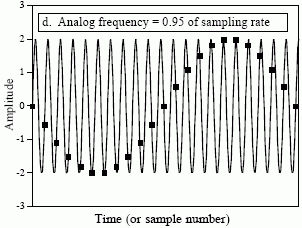
\includegraphics[width=0.35\textwidth]{images/alias-effekt2.png}
		\end{figure}
		\item Nyquist-Frequenz $f_{Nyquist} := \frac{1}{2} f_{abtast}$
		\\ $\Rightarrow$ also $\hat{f}_{signal} < f_{Nyquist}$  \vspace{0.5em}
		% Abtastrate muss größer sein als 2 * die höchste Frequenz die im Signal vorkommt,
		% damit das Signal korrekt rekonstruiert werden kann,
		% sonst kommt es zum Alias-Effekt
	\end{itemize}
\end{frame}

 
